\section{Dynamics in an Asymmetric Hamiltonian} \label{sec:asymham}

\subsection{3-Site Hamiltonian}  \label{sub:hamiltonian}

Instead of a Floquet or quantum circuit system, we can consider one with a time-independent Hamiltonian, for a finite number of dimensions at each site. We can choose a Hamiltonian based on how uneven its dynamics are. For example, the three-site swap $S_{123}$ is a unitary operator such that 
\begin{align}
S_{123}\psi_1\psi_2\psi_3 =\psi_2\psi_3\psi_1, \label{eqn:condition}
\end{align}
where the position of the wavefunction denotes the site on which it sits. 

One way to build the three site swap gate is in a Floquet system, out of two site swap gates $S_{123} = S_{23}S_{12}$. However it is also possible to build it out of a time-independent Hamiltonian, so that $U(1) = \e^{-iH_3} = S_{123}$. This is possible by either taking the matrix-log of $S_{123}$ or by considering the eigenstates and corresponding eigenvalues. 

For a spin-$\half$ system, there will be 8 states, which can be decomposed into a spin-$\frac{3}{2}$ subspace with 4 states and 2 spin-$\half$ subspaces with 2 states each. The eigenstates will be states in which individual particle states differ only by phases. There are four states that should not change in time and therefore have 0 energy. Before normalization these are
\begin{align}
\ket{000},\quad \ket{100}+\ket{010}+\ket{001},\nn
\ket{111},\quad \ket{011}+\ket{101}+\ket{110}.\label{eqn:zero}
\end{align}
Of the four other states, two should have positive energy and two should have negative energy. Since $U(3)=1$, their energies should be $E_\pm = \pm\frac{2\pi}{3}$ so they pick up a phase $\phi_\pm =\e^{-iE_\pm} = \e^{\mp i\frac{2\pi}{3}}$. Using condition~\ref{eqn:condition}, we can show that the positive energy states are
\begin{align}
&\ket{100} + \phi_-\ket{010} + \phi_+\ket{001},\nn
&\ket{011} + \phi_-\ket{101} + \phi_+\ket{110},\label{eqn:plus}
\end{align}
while the negative energy states are 
\begin{align}
&\ket{100} + \phi_+\ket{010} + \phi_-\ket{001},\nn
&\ket{011} + \phi_+\ket{101} + \phi_-\ket{110}.\label{eqn:minus}
\end{align}

In matrix notation, with basis states $\ket{000},\,\ket{001},\,\ket{010},$ etc, the hamiltonian is 
\begin{align}
H_3 = T\; \text{diag}(0,0,0,0,E_+,E_+,E_-,E_-)\; T^\dag,
\end{align}
where $T$ is the transformation matrix suggested by~\ref{eqn:zero}, \ref{eqn:plus}, and~\ref{eqn:minus},
\begin{align}
T = \th{\sqrt{3}}\begin{bmatrix}
\sqrt{3} & 0 & 0 & 0        & 0      & 0      & 0      & 0      \\
0        & 1 & 0 & 0        & \phi_+ & 0      & \phi_- & 0      \\
0        & 1 & 0 & 0        & \phi_- & 0      & \phi_+ & 0      \\
0        & 0 & 1 & 0        & 0      & 1      & 0      & 1      \\
0        & 1 & 0 & 0        & 1      & 0      & 1      & 0      \\
0        & 0 & 1 & 0        & 0      & \phi_- & 0      & \phi_+ \\
0        & 0 & 1 & 0        & 0      & \phi_+ & 0      & \phi_- \\
0        & 0 & 0 & \sqrt{3} & 0      & 0      & 0      & 0
\end{bmatrix}
\end{align}
Altogether
\begin{align}
H_3 = \frac{2\pi i}{\sqrt{3}}\begin{bmatrix}
0 & 0  & 0  & 0  & 0  & 0  & 0  & 0 \\
0 & 0  & 1  & 0  & -1 & 0  & 0  & 0 \\
0 & -1 & 0  & 0  & 1  & 0  & 0  & 0 \\
0 & 0  & 0  & 0  & 0  & -1 & 1  & 0 \\
0 & 1  & -1 & 0  & 0  & 0  & 0  & 0 \\
0 & 0  & 0  & 1  & 0  & 0  & -1 & 0 \\
0 & 0  & 0  & -1 & 0  & 1  & 0  & 0 \\
0 & 0  & 0  & 0  & 0  & 0  & 0  & 0 \\
\end{bmatrix}
\end{align}

This hamiltonian should be symmetric under a simultaneous rotation of all three spins, so that it can be written as $H_3(\bm{\sigma}_1,\,\bm{\sigma}_2 ,\,\bm{\sigma}_3)$. It should be antisymmetric under the interchange of any two spins (equivalent to reversing the direction of propagation). The only function of three vectors that has this property is the triple product $H_3= \bm{\sigma}_1\cdot\left(\bm{\sigma}_2 \times\bm{\sigma}_3\right)$.

%Note that this is equivalent to
%\begin{align}
%H &= \bm{\sigma}_1\cdot\left(\bm{\sigma}_2 \times\bm{\sigma}_3\right) \nn
% &= \sigma_{1,1}\otimes\sigma_{2,2}\otimes{\sigma}_{3,3} - {\sigma}_{1,1}
%	\otimes\sigma_{2,3}\otimes\sigma_{3,2} + \sigma_{1,2}\otimes{\sigma}_{2,3} \otimes {\sigma}_{3,1}-\cdots
%\end{align}

Exponentiating the hamiltonian gives the time evolution operator for one time step
\begin{align}
U(1) = \e^{-iH_3} = \begin{bmatrix}
1 & 0 & 0 & 0 & 0 & 0 & 0 & 0 \\
0 & 0 & 1 & 0 & 0 & 0 & 0 & 0 \\
0 & 0 & 0 & 0 & 1 & 0 & 0 & 0 \\
0 & 0 & 0 & 0 & 0 & 0 & 1 & 0 \\
0 & 1 & 0 & 0 & 0 & 0 & 0 & 0 \\
0 & 0 & 0 & 1 & 0 & 0 & 0 & 0 \\
0 & 0 & 0 & 0 & 0 & 1 & 0 & 0 \\
0 & 0 & 0 & 0 & 0 & 0 & 0 & 1
\end{bmatrix}
\end{align}
This has the properties of of condition~\ref{eqn:condition}. Furthermore, application three times gives $U(3) = 1$. The hamiltonian commutes with the total spin-Z operator $S_Z = \text{diag}(\frac{3}{2}, \frac{1}{2}, \frac{1}{2}, -\frac{1}{2}, \frac{1}{2}, -\frac{1}{2}, -\frac{1}{2}, -\frac{3}{2})$ so total spin-Z is conserved. It also commutes with the other components of spin and therefore also total spin $S^2$.

If the system starts in a computational basis state, for example $\ket{100}$, the coefficients for the other states with equal total spin-Z will both change from 0 before the states becomes $\ket{010}$ at time 1, as in figure~\ref{fig:timeevol}.
\begin{figure}
	\centering
	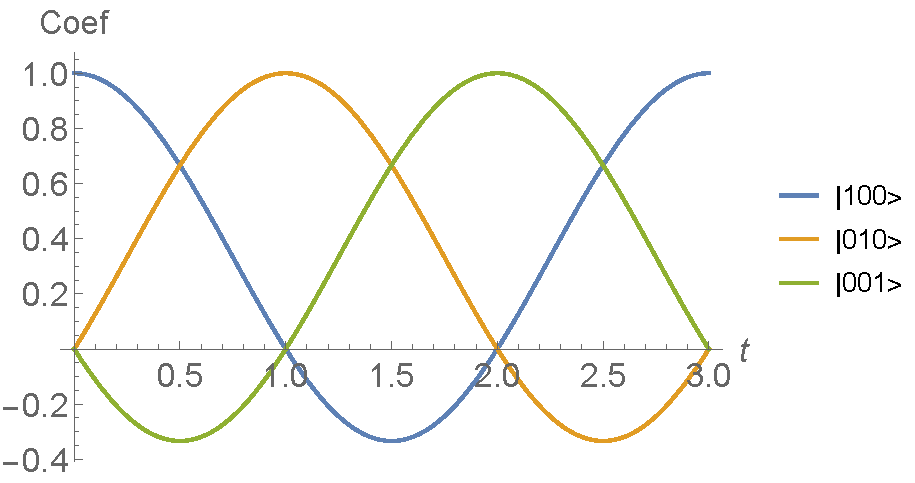
\includegraphics[width=.5\textwidth]{timeevol}
	\caption{Evolution of coefficients if the system starts in state $\ket{100}$.}
	\label{fig:timeevol}
\end{figure}

\subsection{Multi-Site Hamiltonian} \label{sub:multistate}

The 3-site system is integrable, and furthermore is not large enough to effectively study operator spreading.

\subsubsection{Construction} \label{subsub:construction} 

There are multiple ways to extend this hamiltonian to a chain of $L= 2n+1$ spins. Like building $S_{123}$ out of two-site swaps we can treat the larger system as a Floquet system, successively applying $H_3$ to each triplet of spins. We can define a similar hamiltonian by putting the 3-site hamiltonian simultaneously on sites 1-3, sites 3-5, etc. For $n=2$, this is
\begin{align}
H_5 = H_3\otimes\mathbb{I}_2 + \mathbb{I}_2\otimes H_3.
\end{align} 
This hamiltonian still preserves each component of total spin. 

Starting in $\ket{00001}$, the coefficients follow the pattern of figure~\ref{fig:timeevol5}. At first the evolution is similar to the $n=1$ case, with $\ket{10000}$ and then $\ket{01000}$ reaching near maximal. The coefficient of $\ket{00001}$ is 
\begin{align}
\frac{1}{10} \left(3 \cos \left(\frac{2}{3} \sqrt{\frac{5}{3}} \pi  t\right)+5 \cos \left(\frac{2 \pi  t}{3 \sqrt{3}}\right)+2\right)
\end{align} 
which is shown in figure~\ref{fig:onecoef}. Although it appears to be quasi-periodic, it cannot ever reach 1 for $t\ne 0$ or be truly periodic because its time coefficients are not rationally related.

\begin{figure}
	\centering
	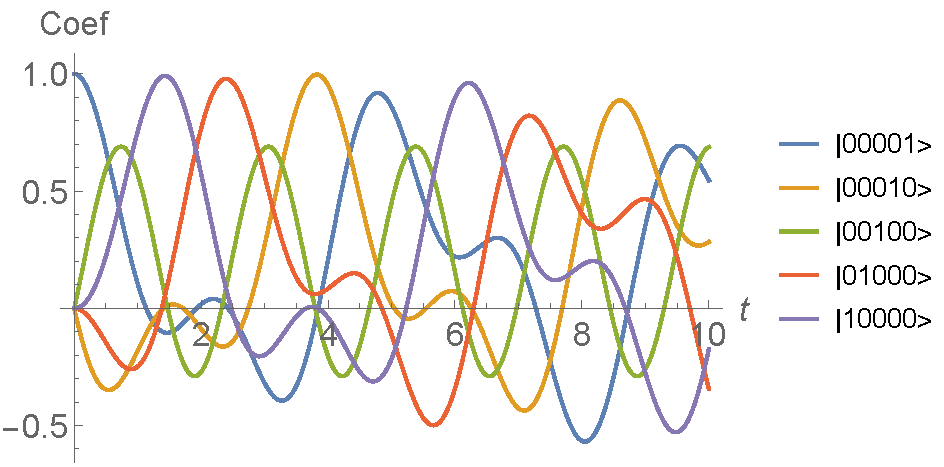
\includegraphics[width=.5\textwidth]{timeevol5}
	\caption{Evolution of coefficients if the system starts in state $\ket{00001}$.}
	\label{fig:timeevol5}
\end{figure}

\begin{figure}
	\centering
	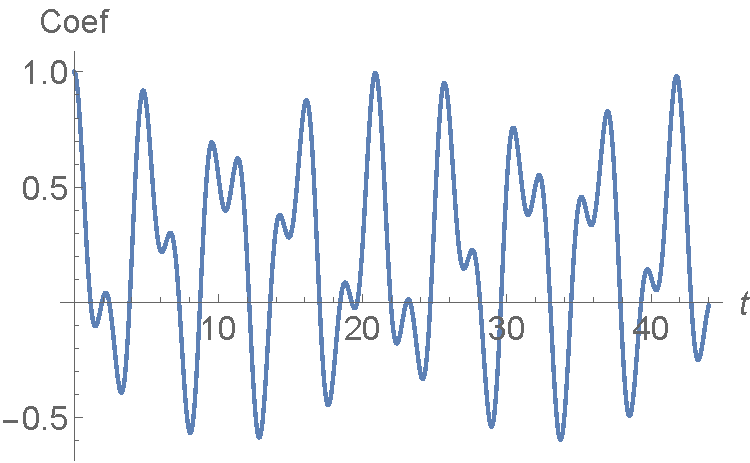
\includegraphics[width=.5\textwidth]{onecoef}
	\caption{Coefficient for $\ket{00001}$ when that is the starting state.}
	\label{fig:onecoef}
\end{figure}

%The coefficient for $\ket{00100}$ does not fit the pattern. It does not reach maximum at the right time and it does have a periodic structure. Furthermore, when the starting state is $\ket{00010}$ the problematic state is still $\ket{00100}$, probably because of the chaining mechanism. When the starting state is $\ket{00100}$ the coefficients for $\ket{10000}$ and $\ket{00001}$ always vanish. The next chaining method to try will be to have $2n$ spins, and to have the first spin complete the last trio.

\subsubsection{Pauli String Weight} \label{subsub:operator_dynamics}  

We can study the operator dynamics of this system by extending to large $L$ and evolving operators that are identities on all sites except one end. Since the hamiltonian is SO(3) symmetric, it does not matter if the perturbation is $X$, $Y$, or $Z$. For convenience, we will use $Z$. We can then study the weight of strings that end at each site $i$, $W(t; i)$.

For the forward-propagating wave, with $A(t=0) = Z_0 = Z\otimes \mathbb{I} \otimes \mathbb{I} \cdots$, the weight starts on site 0 and peaks at even sites. The successive peaks fall off in size but dominate the Pauli strings until the last site takes over (figure~\ref{fig:L11end3n20front}). This is possibly because 

For the backward-propagating waves $(A(t=0)=Z_{L-1})$, the initial decaying signal is more difficult to make out but still present. It is dominated by a large weight of sites that start on site 9 around $t=1$. By $t = 3$ the first site has started to dominate the Pauli weights.

\begin{figure}
	\centering
	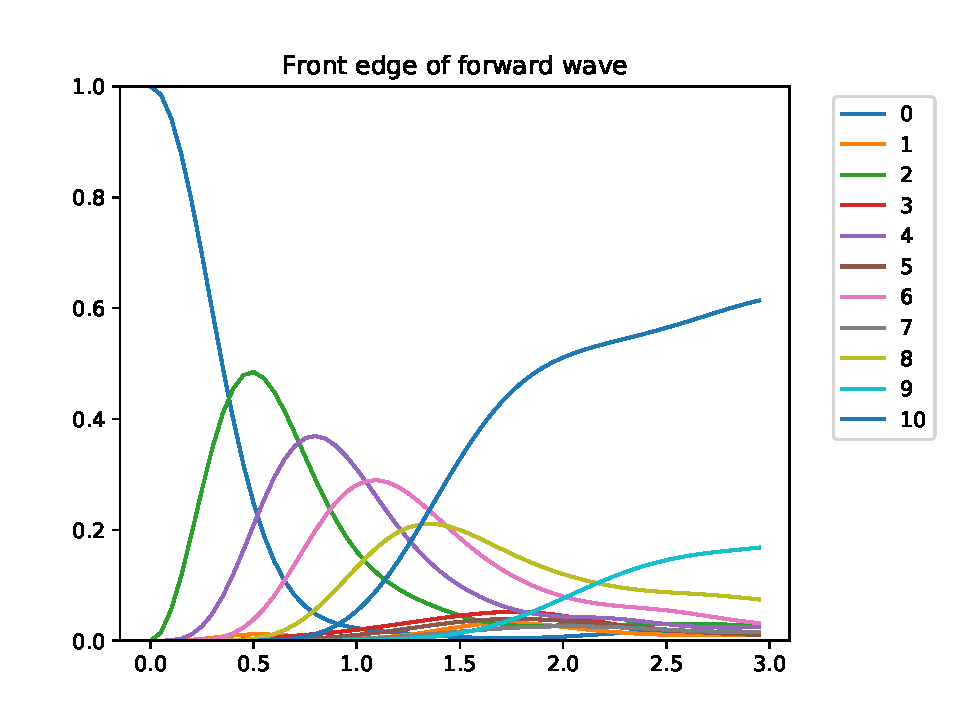
\includegraphics[width=.7\textwidth]{L11end3n20front}
	\caption{Weight of operators that end on site $i$.}
	\label{fig:L11end3n20front}
\end{figure}
\begin{figure}
	\centering
	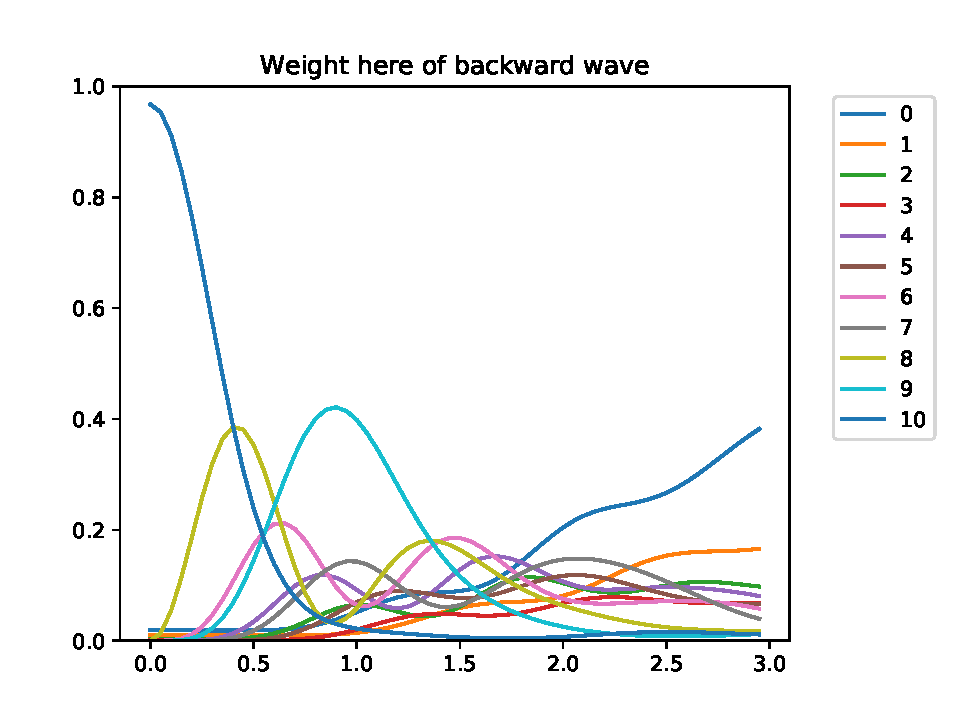
\includegraphics[width=.7\textwidth]{L11end3n20back}
	\caption{Weight of operators that begin on site $i$.}
	\label{fig:L11end3n20back}
\end{figure}

The initial behavior also matches the $L=9$ case. For forward propagation the initial behavior is $W(t;i) = a\e^{bt}$ with $a,b$ given by\dots Figure~\ref{fig:L11end1n60fore} shows this behavior, while figure~\ref{fig:L11end1n60back} shows the analogous behavior for the backward propagating wave. 

\begin{figure}
	\centering
	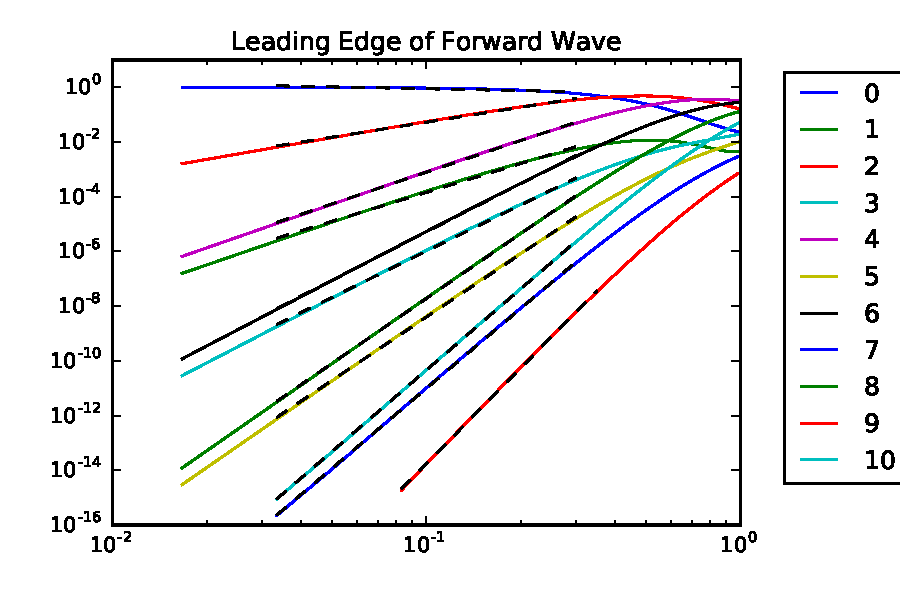
\includegraphics[width=.7\textwidth]{L11end1n60fore}
	\caption{Early-time leading edge weights for forward propagating wave.}
	\label{fig:L11end1n60fore}
\end{figure}
\begin{figure}
	\centering
	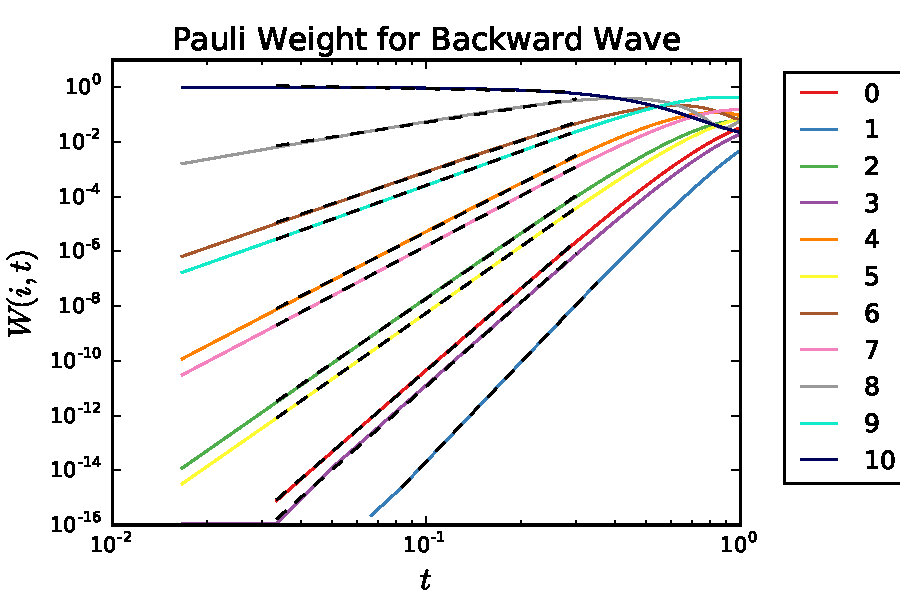
\includegraphics[width=.7\textwidth]{L11end1n60back}
	\caption{Early-time leading edge weights for backward propagating wave.}
	\label{fig:L11end1n60back}
\end{figure}

Here the relevant numbers are\dots
Again, the exponents for even and odd sites increase by one within each group. Pairs of sites separated by 3 are also divergent in the forward case while convergent in the backward case.